\documentclass[10pt, letterpaper]{report}
% !TeX program = xelatex
%==================PREAMBOLO=======================%
\usepackage[utf8]{inputenc}
\usepackage{psvectorian}
\usepackage{pgfplots}
\usepackage[Rejne]{fncychap}
\usepackage[export]{adjustbox}
\usepackage[T1]{fontenc}
\usepackage{lmodern}
\usepackage{blindtext}
\usepackage{pdfpages}
\usepackage[shortlabels]{enumitem}
\usepackage{moresize}
\usepackage{stmaryrd}
\usepackage{graphicx} % Required for inserting images
\usepackage{hyperref}
\usepackage{listings}
\usepackage{mathtools}
\usepackage[table,xcdraw]{xcolor}
\usepackage{amssymb}
\usepackage{amsmath}
\usepackage[english]{babel}
\usepackage{nicefrac, xfrac}
\usepackage{tikz}
\usepackage{tikz-3dplot}
\usepackage{tikz-cd}
\usepackage{mathrsfs} 
\usepackage{titletoc}
\usepackage{fancyhdr}
\usepackage{psvectorian,lipsum}
\usepackage{fourier-orns}
\usepackage{lipsum}
\usepackage{wrapfig}
\usepackage{multicol}
\usepackage{titlesec}
\usepackage[paper=a4paper,left=25mm,right=25mm,bottom=25mm,top=25mm]{geometry}
\usepackage[most]{tcolorbox}
\usepackage{amsfonts}

\definecolor{light-gray}{gray}{0.95}
\definecolor{cop}{HTML}{f7ecd7}
\definecolor{copAut}{HTML}{ababab}
\definecolor{copAut2}{HTML}{c3c3e6}
\definecolor{purcop}{HTML}{d0d3db}
\definecolor{sapienza}{HTML}{660f1d}
\definecolor{lightSapienza}{HTML}{e3d3d5}
\definecolor{darkgreen}{HTML}{008000}
\definecolor{cartaRiciclata}{HTML}{fcfcf7}
\newcommand{\quadBrack}[1]{ \llbracket #1 \rrbracket }
\newcommand{\redText}[1]{\color{red}#1\color{black}}
\newcommand{\sapText}[1]{\color{sapienza}#1\color{black}}
\newcommand{\blueText}[1]{\color{blue}#1\color{black}}
\newcommand{\greenText}[1]{\color{darkgreen}#1\color{black}}
\newcommand{\code}[1]{\colorbox{light-gray}{\texttt{#1}}}
\newcommand{\codee}[1]{\colorbox{white}{\texttt{#1}}}
\newcommand{\K}{{\mathbb K}}
\newcommand{\notimplies}{%
  \mathrel{{\ooalign{\hidewidth$\not\phantom{=}$\hidewidth\cr$\implies$}}}}
\newcommand{\flowerLine}{ \begin{center}\decofourleft\hphantom{ }\decoone\hphantom{ }\decofourright\hphantom{}\hphantom{aa}
\decofourleft\hphantom{ }\decoone\hphantom{ }\decofourright\hphantom{}\hphantom{aa}
\decofourleft\hphantom{ }\decoone\hphantom{ }\decofourright\hphantom{}\hphantom{aa}
\decofourleft\hphantom{ }\decoone\hphantom{ }\decofourright\hphantom{}\hphantom{aa} 
\decofourleft\hphantom{ }\decoone\hphantom{ }\decofourright\hphantom{}\hphantom{aa}
\decofourleft\hphantom{ }\decoone\hphantom{ }\decofourright\hphantom{}\hphantom{aa}
\decofourleft\hphantom{ }\decoone\hphantom{ }\decofourright\hphantom{}\hphantom{aa}
\decofourleft\hphantom{ }\decoone\hphantom{ }\decofourright\hphantom{}\hphantom{aa}
\decofourleft\hphantom{ }\decoone\hphantom{ }\decofourright\hphantom{}\hphantom{aa}
\end{center}}
\definecolor{g}{RGB}{60, 50, 50}
\newcommand{\textg}[1]{\color{g}{\textbf{#1}}\color{black}}
\newcommand{\teo}[1]{{\large\color{sapienza}\textbf{Teorema #1 :\hphantom{a}}}}
\newcommand{\defi}[1]{{\large\color{sapienza}\textbf{Definizione #1 :\hphantom{a}}}}
\newcommand{\claim}[1]{{\color{sapienza}\textbf{Claim #1 :\hphantom{a}}}}
\newcommand{\lemma}[1]{{\color{sapienza}\textbf{Lemma #1 :\hphantom{a}}}}
\newcommand{\dimo}[1]{{\color{sapienza}\textbf{Dimostrazione #1 :\hphantom{a}}}}
\newcommand{\prop}[1]{{\color{sapienza}\textbf{Proposizione #1 :\hphantom{a}}}}
\newcommand\greybox[1]{%
  \vskip\baselineskip%
  \par\noindent\colorbox{light-gray}{%
    \begin{minipage}{\textwidth}#1\end{minipage}%
  }%
  \vskip\baselineskip%
}
\newcommand\sapbox[1]{%
  \vskip\baselineskip%
  \par\noindent\colorbox{lightSapienza}{%
    \begin{minipage}{\textwidth}#1\end{minipage}%
  }%
  \vskip\baselineskip%
}
\newcommand{\ridFunc}{{f:\Sigma^*\rightarrow \Sigma^*}}
\newcommand{\rid}{{\le_m^P}}
\newcommand{\Z}{{\mathbb Z}}
\newcommand{\blank}{{\sqcup}}
\newcommand{\Prob}{{\mathbb P}}
\newcommand{\R}{{\mathbb R}}
\newcommand{\VA}{{\mathbb E}}
\newcommand{\btheta}{{\boldsymbol{\theta}}}
\newcommand{\btau}{{\boldsymbol{\tau}}}
\newcommand{\bomega}{{\boldsymbol{\omega}}}
\newcommand{\bmu}{{\boldsymbol{\mu}}}
\newcommand{\brho}{{\boldsymbol{\rho}}}
\newcommand{\N}{{\mathbb N}}
\newcommand{\quat}{{\mathbb H}}
\newcommand{\C}{{\mathbb C}}
\newcommand{\Sn}{{\mathcal S_n}}
\newcommand{\An}{{\mathcal A_n}}
\newcommand{\E}{{\mathcal E}}
\newcommand{\B}{{\mathcal B}}
\newcommand{\mcm}{{\text{mcm}}}
\newcommand{\rg}{{\text{rg}}}
\newcommand{\dq}{{\dot{\mathbf q}}}
\newcommand{\de}{{\dot{\mathbf e}}}
\newcommand{\dy}{{\dot{\mathbf y}}}
\newcommand{\ddq}{{\ddot{\mathbf q}}}
\newcommand{\ddy}{{\ddot{\mathbf y}}}
\newcommand{\ve}{{\bar v}}
\newcommand{\spaz}{{\text{\hphantom{aa}}}}
\newcommand{\MCD}{{\text{MCD}}}
\newcommand{\tc}{{\text{ tale che }}}
\newcommand{\supp}{{\text{Supp}}}
\newcommand{\acc}{\\\hphantom{}\\}
\newcommand{\esempio}[1]{{\acc\large\color{sapienza}\textbf{Esempio #1 \hphantom{a}}\acc}}
\newcommand{\bra}[1]{\langle #1 \rangle}
\newcommand{\aut}{{\text{Aut}}}
\newcommand{\Span}{{\text{Span}}}
\newcommand{\End}{{\text{End}}}
\newcommand{\cen}{{\text{Centro}}}
\newcommand{\norm}{{\unlhd}}
\newcommand{\ciclS}{{\left \langle }}
\newcommand{\ciclE}{{\right \rangle }}
\newcommand{\boxedMath}[1]{\begin{tabular}{|c|}\hline \texttt{#1} \\ \hline\end{tabular} :} 
\newcommand{\shell}[1]{\colorbox{black}{\textcolor{white}{\texttt{#1}}}}
\newcommand{\eqImportante}[1]{\begin{center}\huge\lefthand\hphantom{a}
    \normalsize\texttt{#1}
    \hphantom{aaa}\huge\righthand\end{center}}

\fancyhf{}
\pagestyle{fancy}
\usepackage{pgf-pie}  
\usetikzlibrary{positioning}

\renewcommand{\headrule}{%
\vspace{-8pt}\hrulefill
\raisebox{-2.1pt}{\quad\decothreeleft\decotwo\decothreeright\quad}\hrulefill}

%sta roba serve per il codice C
\definecolor{mGreen}{rgb}{0,0.6,0}
\definecolor{mGray}{rgb}{0.5,0.5,0.5}
\definecolor{mPurple}{rgb}{0.58,0,0.82}
\definecolor{backgroundColour}{rgb}{0.95,0.95,0.92}

\lstdefinestyle{CStyle}{
    backgroundcolor=\color{backgroundColour},   
    commentstyle=\color{mGreen},
    keywordstyle=\color{magenta},
    numberstyle=\tiny\color{mGray},
    stringstyle=\color{mPurple},
    basicstyle=\footnotesize,
    breakatwhitespace=false,         
    breaklines=true,                 
    captionpos=b,                    
    keepspaces=true,                 
    numbers=left,                    
    numbersep=5pt,                  
    showspaces=false,                
    showstringspaces=false,
    showtabs=false,                  
    tabsize=2,
    language=C
}
\lstdefinestyle{CppStyle}{
    backgroundcolor=\color{backgroundColour},   
    commentstyle=\color{mGreen}\ttfamily,
    morecomment=[l][\color{magenta}]{\#}
    keywordstyle=\color{blue}\ttfamily,
    numberstyle=\tiny\color{mGray},
    stringstyle=\color{red}\ttfamily,
    basicstyle=\ttfamily,
    breakatwhitespace=false,         
    breaklines=true,                 
    captionpos=b,                    
    keepspaces=true,                 
    numbers=left,                    
    numbersep=5pt,                  
    showspaces=false,                
    showstringspaces=false,
    showtabs=false,                  
    tabsize=2,
    language=C
}
\lstset{language=C++,
                basicstyle=\ttfamily,
                keywordstyle=\color{blue}\ttfamily,
                stringstyle=\color{red}\ttfamily,
                commentstyle=\color{green}\ttfamily,
                morecomment=[l][\color{magenta}]{\#}
}
%fine roba che serve per il codice C
\usepackage{minted}
\usepackage[scaled]{helvet}
\usepackage{needspace}
\tcbuselibrary{theorems}

%TEOREMI ECC 
\newtcbtheorem[number within=section]{boxdefinition}{Definition}{
    enhanced,
    before skip=15pt, after skip=15pt,
    colback=white, % Fondo bianco per il testo
    colframe=sapienza!50!black!30, % Colore del bordo (verde chiaro/grigio)
    fonttitle=\bfseries,
    coltitle=black,
    % Stile della "linguetta" superiore
    attach boxed title to top left={xshift=10mm, yshift=-3.5mm, yshifttext=-1mm},
    boxed title style={
        colframe=sapienza!50!black!30,
        arc=3mm,
        outer arc=3mm,
        left=10pt, right=10pt,
        top=2pt, bottom=2pt,
        % Sfumatura di verde (gradient) come nell'immagine
        interior style={left color=sapienza!20, right color=sapienza!40}
    },
    % Arrotondamento del box principale
    arc=4mm,
    separator sign none, % Rimuove i due punti automatici se vuoi scriverli tu nel titolo
    description font=\normalfont\bfseries,
    description delimiters={: }{ } % Formatta il titolo come "Definition 2.1: Titolo"
}{def}

\newtcbtheorem[number within=section]{boxtheorem}{Theorem}{
    enhanced,
    before skip=15pt, after skip=15pt,
    colback=white, % Fondo bianco per il testo
    colframe=sapienza!50!black!30, % Colore del bordo (verde chiaro/grigio)
    fonttitle=\bfseries,
    coltitle=black,
    % Stile della "linguetta" superiore
    attach boxed title to top left={xshift=10mm, yshift=-3.5mm, yshifttext=-1mm},
    boxed title style={
        colframe=sapienza!50!black!30,
        arc=3mm,
        outer arc=3mm,
        left=10pt, right=10pt,
        top=2pt, bottom=2pt,
        % Sfumatura di verde (gradient) come nell'immagine
        interior style={left color=sapienza!20, right color=sapienza!40}
    },
    % Arrotondamento del box principale
    arc=4mm,
    separator sign none, % Rimuove i due punti automatici se vuoi scriverli tu nel titolo
    description font=\normalfont\bfseries,
    description delimiters={: }{ } % Formatta il titolo come "Definition 2.1: Titolo"
}{def}

\newtcbtheorem[number within=section]{boxproposition}{Proposition}{
    enhanced,
    before skip=15pt, after skip=15pt,
    colback=white, % Fondo bianco per il testo
    colframe=sapienza!50!black!30, % Colore del bordo (verde chiaro/grigio)
    fonttitle=\bfseries,
    coltitle=black,
    % Stile della "linguetta" superiore
    attach boxed title to top left={xshift=10mm, yshift=-3.5mm, yshifttext=-1mm},
    boxed title style={
        colframe=sapienza!50!black!30,
        arc=3mm,
        outer arc=3mm,
        left=10pt, right=10pt,
        top=2pt, bottom=2pt,
        % Sfumatura di verde (gradient) come nell'immagine
        interior style={left color=sapienza!30, right color=sapienza!50}
    },
    % Arrotondamento del box principale
    arc=4mm,
    separator sign none, % Rimuove i due punti automatici se vuoi scriverli tu nel titolo
    description font=\normalfont\bfseries,
    description delimiters={: }{ } % Formatta il titolo come "Definition 2.1: Titolo"
}{def}

\newtcbtheorem[number within=section]{boxequation}{Equation}{
    enhanced,
    before skip=15pt, after skip=15pt,
    colback=white, % Fondo bianco per il testo
    colframe=sapienza!50!black!30, % Colore del bordo (verde chiaro/grigio)
    fonttitle=\bfseries,
    coltitle=black,
    % Stile della "linguetta" superiore
    attach boxed title to top left={xshift=10mm, yshift=-3.5mm, yshifttext=-1mm},
    boxed title style={
        colframe=sapienza!50!black!30,
        arc=3mm,
        outer arc=3mm,
        left=10pt, right=10pt,
        top=2pt, bottom=2pt,
        % Sfumatura di verde (gradient) come nell'immagine
        interior style={left color=sapienza!30, right color=sapienza!50}
    },
    % Arrotondamento del box principale
    arc=4mm,
    separator sign none, % Rimuove i due punti automatici se vuoi scriverli tu nel titolo
    description font=\normalfont\bfseries,
    description delimiters={: }{ } % Formatta il titolo come "Definition 2.1: Titolo"
}{def}

\newtcbtheorem[number within=section]{boxlemma}{Lemma}{
    enhanced,
    before skip=15pt, after skip=15pt,
    colback=white, % Fondo bianco per il testo
    colframe=sapienza!50!black!30, % Colore del bordo (verde chiaro/grigio)
    fonttitle=\bfseries,
    coltitle=black,
    % Stile della "linguetta" superiore
    attach boxed title to top left={xshift=10mm, yshift=-3.5mm, yshifttext=-1mm},
    boxed title style={
        colframe=sapienza!50!black!30,
        arc=3mm,
        outer arc=3mm,
        left=10pt, right=10pt,
        top=2pt, bottom=2pt,
        % Sfumatura di verde (gradient) come nell'immagine
        interior style={left color=sapienza!30, right color=sapienza!50}
    },
    % Arrotondamento del box principale
    arc=4mm,
    separator sign none, % Rimuove i due punti automatici se vuoi scriverli tu nel titolo
    description font=\normalfont\bfseries,
    description delimiters={: }{ } % Formatta il titolo come "Definition 2.1: Titolo"
}{def}

\newtcbtheorem[number within=section]{boxobservation}{Observation}{
    enhanced,
    before skip=15pt, after skip=15pt,
    colback=white, % Fondo bianco per il testo
    colframe=sapienza!50!black!30, % Colore del bordo (verde chiaro/grigio)
    fonttitle=\bfseries,
    coltitle=black,
    % Stile della "linguetta" superiore
    attach boxed title to top left={xshift=10mm, yshift=-3.5mm, yshifttext=-1mm},
    boxed title style={
        colframe=sapienza!50!black!30,
        arc=3mm,
        outer arc=3mm,
        left=10pt, right=10pt,
        top=2pt, bottom=2pt,
        % Sfumatura di verde (gradient) come nell'immagine
        interior style={left color=sapienza!30, right color=sapienza!50}
    },
    % Arrotondamento del box principale
    arc=4mm,
    separator sign none, % Rimuove i due punti automatici se vuoi scriverli tu nel titolo
    description font=\normalfont\bfseries,
    description delimiters={: }{ } % Formatta il titolo come "Definition 2.1: Titolo"
}{def}

\newtcbtheorem[number within=section]{boxpostulate}{Postulate}{
    enhanced,
    before skip=15pt, after skip=15pt,
    colback=white, % Fondo bianco per il testo
    colframe=sapienza!50!black!30, % Colore del bordo (verde chiaro/grigio)
    fonttitle=\bfseries,
    coltitle=black,
    % Stile della "linguetta" superiore
    attach boxed title to top left={xshift=10mm, yshift=-3.5mm, yshifttext=-1mm},
    boxed title style={
        colframe=sapienza!50!black!30,
        arc=3mm,
        outer arc=3mm,
        left=10pt, right=10pt,
        top=2pt, bottom=2pt,
        % Sfumatura di verde (gradient) come nell'immagine
        interior style={left color=sapienza!30, right color=sapienza!50}
    },
    % Arrotondamento del box principale
    arc=4mm,
    separator sign none, % Rimuove i due punti automatici se vuoi scriverli tu nel titolo
    description font=\normalfont\bfseries,
    description delimiters={: }{ } % Formatta il titolo come "Definition 2.1: Titolo"
}{def}

\titleformat{\section}
  {\needspace{3\baselineskip} % <--- Chiede almeno 3 righe di spazio libero
   \fontfamily{phv}\selectfont\huge\bfseries} 
  {\color{sapienza}\fontsize{20}{20}\selectfont\thesection} 
  {12pt} 
  {} 
  [\vspace{2pt}\nopagebreak\color{sapienza!40}\hrule height 3pt]

% Per la Sottosezione
\titleformat{\subsection}
  {\needspace{2\baselineskip} % <--- Chiede almeno 2 righe di spazio libero
   \fontfamily{phv}\selectfont\Large\bfseries} 
  {\color{sapienza}\fontsize{16}{16}\selectfont\thesubsection} 
  {12pt} 
  {} 
  [\vspace{2pt}\nopagebreak\color{sapienza!40}\hrule height 1.5pt]
\newcommand{\titolo}{Computer Vision }

 %TOGLI COMMENTO SE USI XELATEX
%\usepackage{fontspec}
\title{\titolo} %========TITOLO========%
\author{Marco Casu}
\date{\vspace{-5ex}}
\begin{document}

%==================COPERTINA=======================%
\begin{titlepage}
    
\begin{center}
    %TOGLI COMMENTO SE USI XELATEX
   %\setmainfont{Palace Script MT}
   \HUGE Marco Casu\acc
\end{center}
\thispagestyle{empty}
\begin{figure}[h]
    \centering{
        %l'immagine deve avere una risoluzione 2048x2048
        
\includegraphics[width=0.95\textwidth ]{images/Copertina.png}
    }
\end{figure}
\vfill 
\centering 
\includegraphics[width=0.4\textwidth ]{../../preamble/Stemma_sapienza.png} \acc
\centering \Large \color{sapienza}Faculty of Information Engineering, Computer Science and Statistics\\
Department of Computer, Control and Management Engineering\\
Master's degree in Artificial Intelligence and Robotics
\end{titlepage}

%===================FINE COPERTINA======================%
\newpage
%\pagecolor{cartaRiciclata}%\setmainfont{Algerian}
\Large
This document summarizes and presents the topics for the \titolo course for the Master's degree in Artificial Intelligence and Robotics at Sapienza University of Rome. The document is free for any use. If the reader notices any typos, they are kindly requested to report them to the author.
\vfill
\begin{figure}[h!]
    \raggedright
    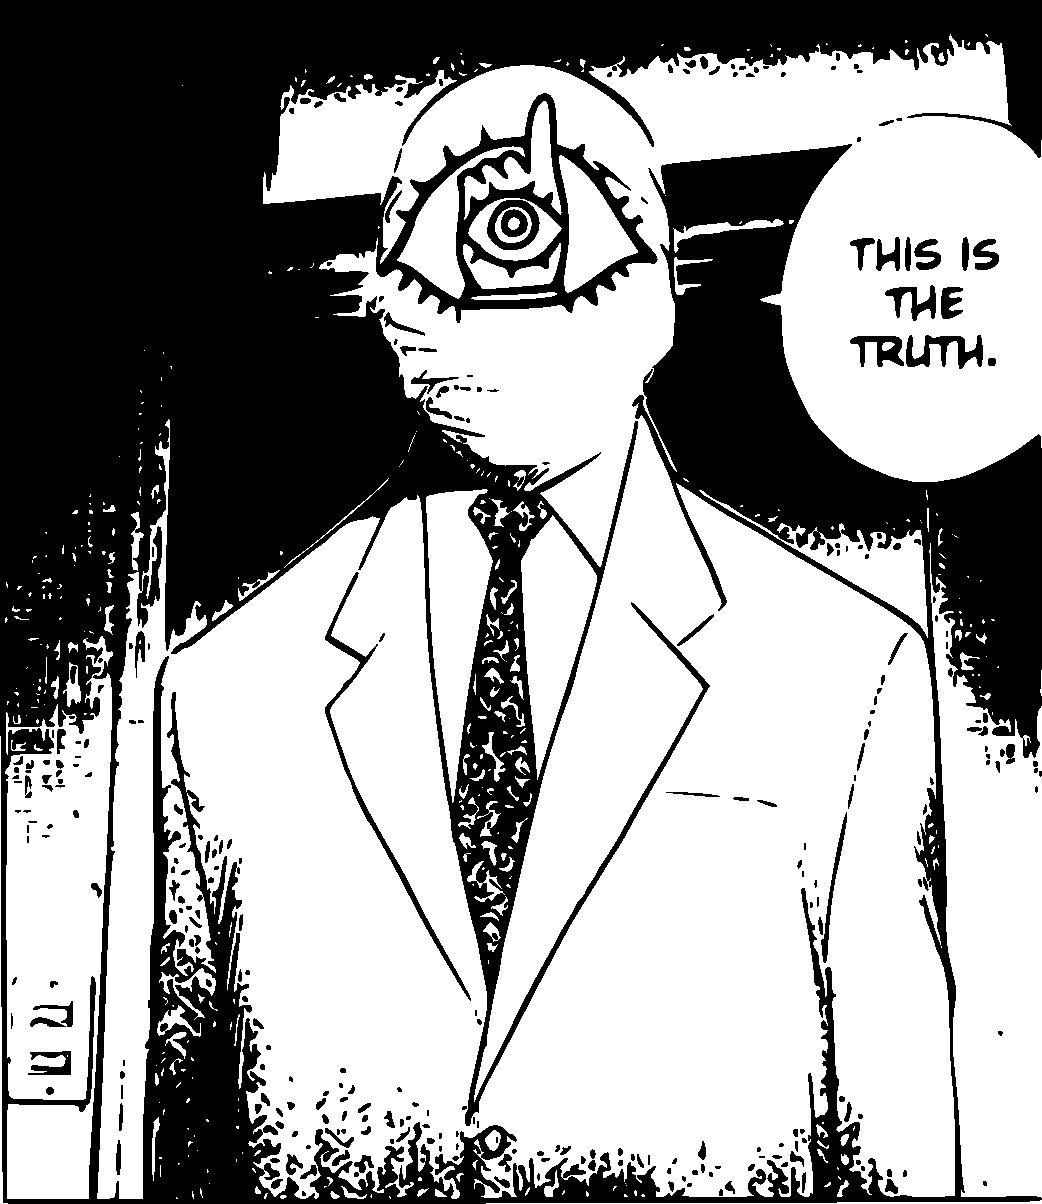
\includegraphics[width=0.4\textwidth,right ]{../../preamble/tomodachi.pdf} 
\end{figure}
\newpage %\setmainfont{Times New Roman}
\normalsize

\tableofcontents 
\newpage

%==================FOOTER e HEADER=======================%
\fancyhf{}
\fancyhead[L]{\nouppercase{\leftmark}}
\fancyhead[R]{Section \thesection}
\fancyfoot[C]{\thepage}
\fancyfoot[L]{\titolo}
\fancyfoot[R]{ Marco Casu}
%\fancyfoot[R]{\setmainfont{Palace Script MT}\huge Marco Casu \setmainfont{Times New Roman}}
%==================FOOTER e HEADER=======================%
\newtheorem{definition}{Definition}
\newtheorem{proposition}{Proposition}
\newtheorem{theorem}{Theorem}
%==================INIZIO======================%
\chapter{Image Processing}
An image is just a grid (matrix) where each entries represents the intensity of that pixel, for example, in grey scale images, each entry is an integer between 0 and 255 (1 byte for pixel), where 0 represents the black, 255 the white, and the other values the scale of greys.
\begin{center}
    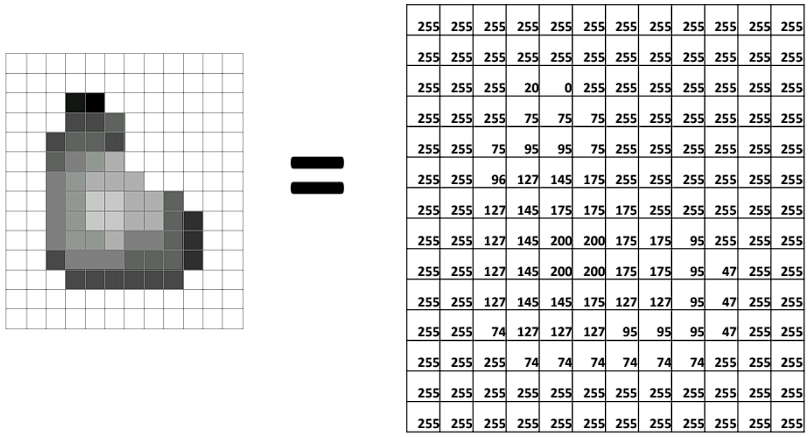
\includegraphics[width=0.6\textwidth ]{images/greys.png} 
\end{center}
In such way a grey scale image can be seen as a function $f:\R^2\rightarrow\R$, for the digital images, the values of the function are restricted to the integers in $[0,255]$ (also the domain is discrete and restricted to the couples of integers). Of course, color images are coded with 3 channels (Red Green Blue), so for each entry there is a triple of integers between 0 and 255 (3 byte).
\begin{center}
    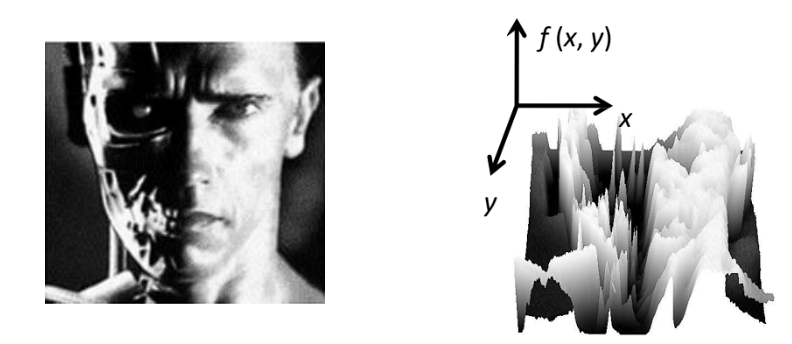
\includegraphics[width=0.6\textwidth ]{images/function_image.png} 
\end{center}

\section{Filtering}
\begin{boxdefinition}{Filter}{}
    a filter is a mathematical algorithm applied to an image to modify its characteristics, highlight certain information or remove disturbances (noise).
\end{boxdefinition}
\begin{figure}[H]
    \center
    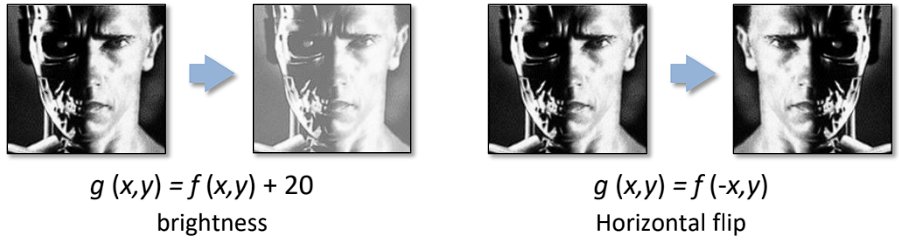
\includegraphics[width=0.6\textwidth ]{images/filters.png} 
    \caption{Example of two filters}
\end{figure}
\subsection{Point Processing}
The first simple filter to consider is the \textbf{Gamma Correction}, this adjust the brightness and contrast in images. The human eye perceives light in a non-linear way, and gamma correction ensures
images appear natural. Human vision is more sensitive to changes in darker tones than in lighter tones.

\redText{TODO}
\subsection{Linear Filtering}
The goal of the filtering procedure is to form a new image whose pixel values are a combination of the original pixel values, this is useful to enhance the image and get useful information from them.

One key example is the noise reduction.
\begin{figure}[H]
    \center
    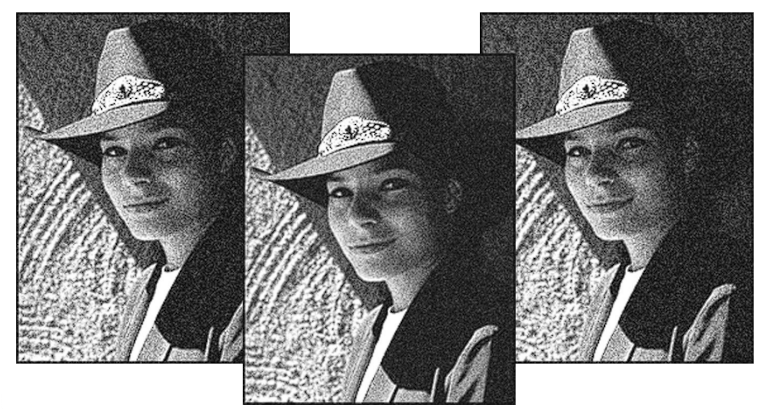
\includegraphics[width=0.5\textwidth ]{images/noise.png} 
    \caption{Noisy image from a camera}
\end{figure}
A \textit{linear filter} replace each pixel of the original images with a new one computed as a combination (weighted sum) of its neighbors, trough the application of the cross-correlation operator or the convolution.

Each linear filter is defined by a \textit{kernel}, a matrix on which we will perform the convolution (or cross correlation) with the original images.
\begin{center}
    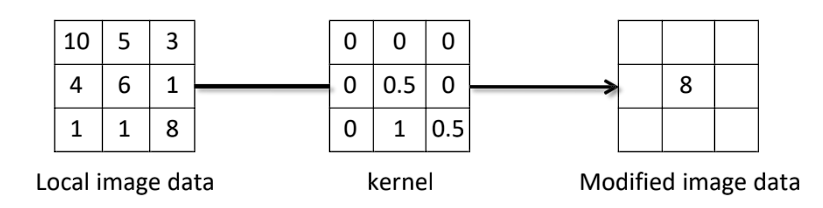
\includegraphics[width=0.6\textwidth ]{images/linearFilter.png} 
\end{center}
\begin{boxdefinition}{Cross Correlation}{}
    The discrete cross correlation operator between two matrices $F$ (the image) and $H$ (the kernel) results in the output matrix $G$ defined as follows\begin{equation}
        G[i,j]=\sum_{u=-k}^k\sum_{v=-k}^k H[u,v]F[i+u,j+v]
    \end{equation}
\end{boxdefinition}
we  write the result of the cross correlation as follows $G=H\otimes F$. The \textbf{Convolution} is similar but the kernel is flipped horizontally and vertically \begin{equation}
        G[i,j]=\sum_{u=-k}^k\sum_{v=-k}^k H[u,v]F[i-u,j-v]
    \end{equation}
we  write the result of the convolution as follows $G=H\star F$. The convolution is commutative and associative.
\begin{center}
    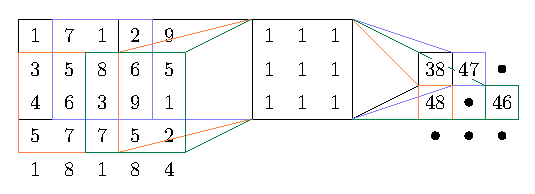
\includegraphics[width=0.5\textwidth ]{images/kernel.eps} 
\end{center}
An example of filter is the \textit{mean filter}, that assign at a given pixel the average of the neighbors, giving a blurry effects. Considering more neighbors will result in a stronger blur.
\begin{center}
    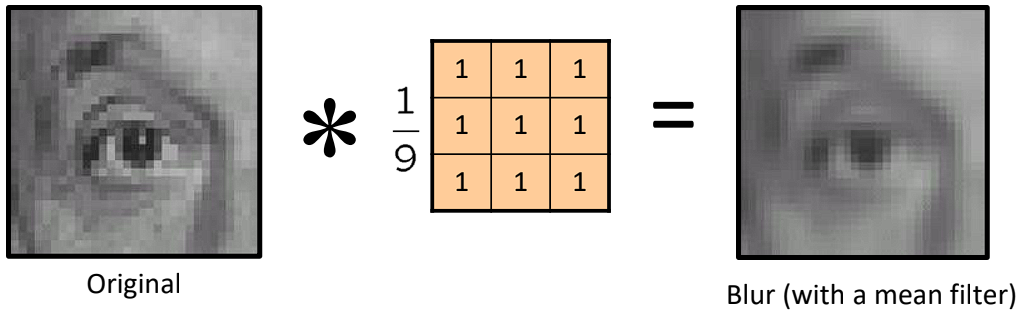
\includegraphics[width=0.6\textwidth ]{images/blur.png} 
\end{center}
a filter is called \textbf{separable} if the kernel can be expressed as the outer product of two vectors, this property makes the application of a filter less expensive from a computational point of view, since the 2D convolution with a separable filter is equivalent to two 1D convolution (with the column and row filters).\begin{equation}
    \begin{bmatrix}
        1&1&1\\ 
        1&1&1\\ 
        1&1&1
    \end{bmatrix}=\begin{bmatrix}
        1\\1\\1
    \end{bmatrix}\cdot\begin{bmatrix}
        1&1&1
    \end{bmatrix}
\end{equation}
if an image have a resolution $m\times n$ and the filter has size $l\times l$:\begin{itemize}
    \item the convolution with a non separable filter needs $l^2mn$ operations 
    \item the convolution with a separable filter needs $2lmn$ operations.
\end{itemize}
A kernel is separable if and only if the matrix has rank 1.\bigskip 

Now we consider a useful non linear filter, the \textbf{Gaussian kernel} is the 2D filter $G_\sigma$ defined as follows:\begin{equation}\label{gaussian_filter}
    G_\sigma[i,j]=\frac{1}{2\pi\sigma^2}\exp\left(-\frac{i^2+j^2}{2\sigma^2}\right)
\end{equation}
\begin{figure}[H]
    \center
    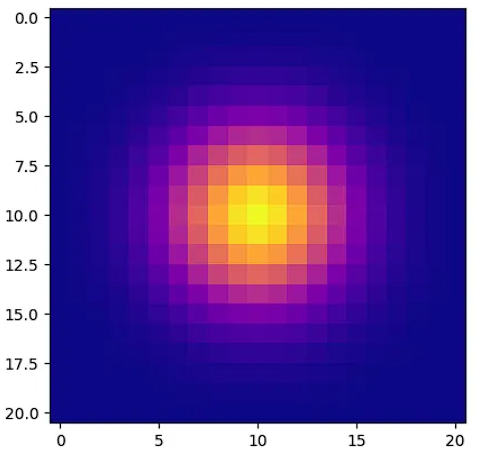
\includegraphics[width=0.3\textwidth ]{images/gaussian_kernel.png} 
    \caption{Heatmap of the Gaussian kernel}
\end{figure}
The Gaussian filter gives a blurry effects, in particular, removes the \textit{high frequencies} from an image (will be explained later). The convolution of two Gaussian filters is still a gaussian filter.
\begin{figure}[H]
    \center
    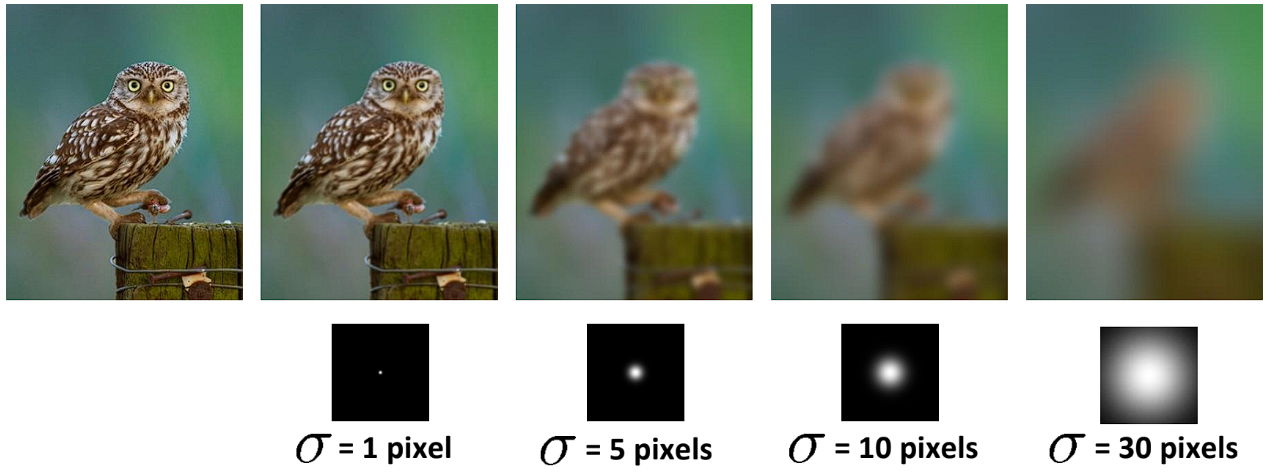
\includegraphics[width=0.8\textwidth ]{images/gaussian_kernel_example.png} 
    \caption{Application of the Gaussian kernel with different values for $\sigma$}
\end{figure}
Another important filter is the \textbf{Sharpening filter}.
\begin{center}
    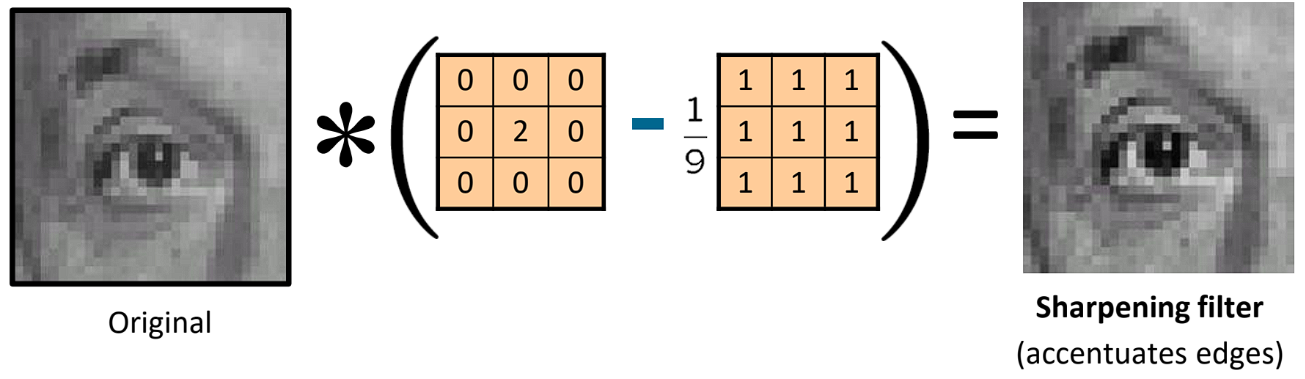
\includegraphics[width=0.6\textwidth ]{images/sharpening.png} 
\end{center}
Is given by the difference between a scaled \textit{impulse} and a mean filter. If we subtract the original images from the sharpened one we obtain an image that represents only the details.
\begin{center}
    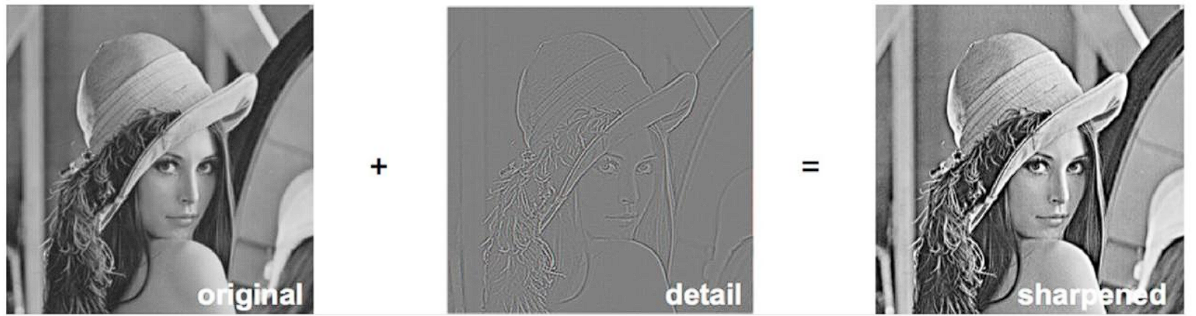
\includegraphics[width=0.6\textwidth ]{images/details.png} 
\end{center}
The sharpening operation can be done with the Gaussian filter instead of the mean one:\begin{equation}
    ((1+\alpha)e-\alpha H)\\ 
\end{equation}
where
\begin{itemize}
    \item $\alpha$ is the value to control how sharpening the filter is 
    \item $H$ is the Gaussian kernel 
    \item $e$ is the unit impulse, matrix with 1 in the center and zero in the other entries\begin{equation}
        \begin{bmatrix}
            0&0&0\\
            0&1&0\\
            0&0&0
        \end{bmatrix}.
    \end{equation}
\end{itemize}
\begin{center}
    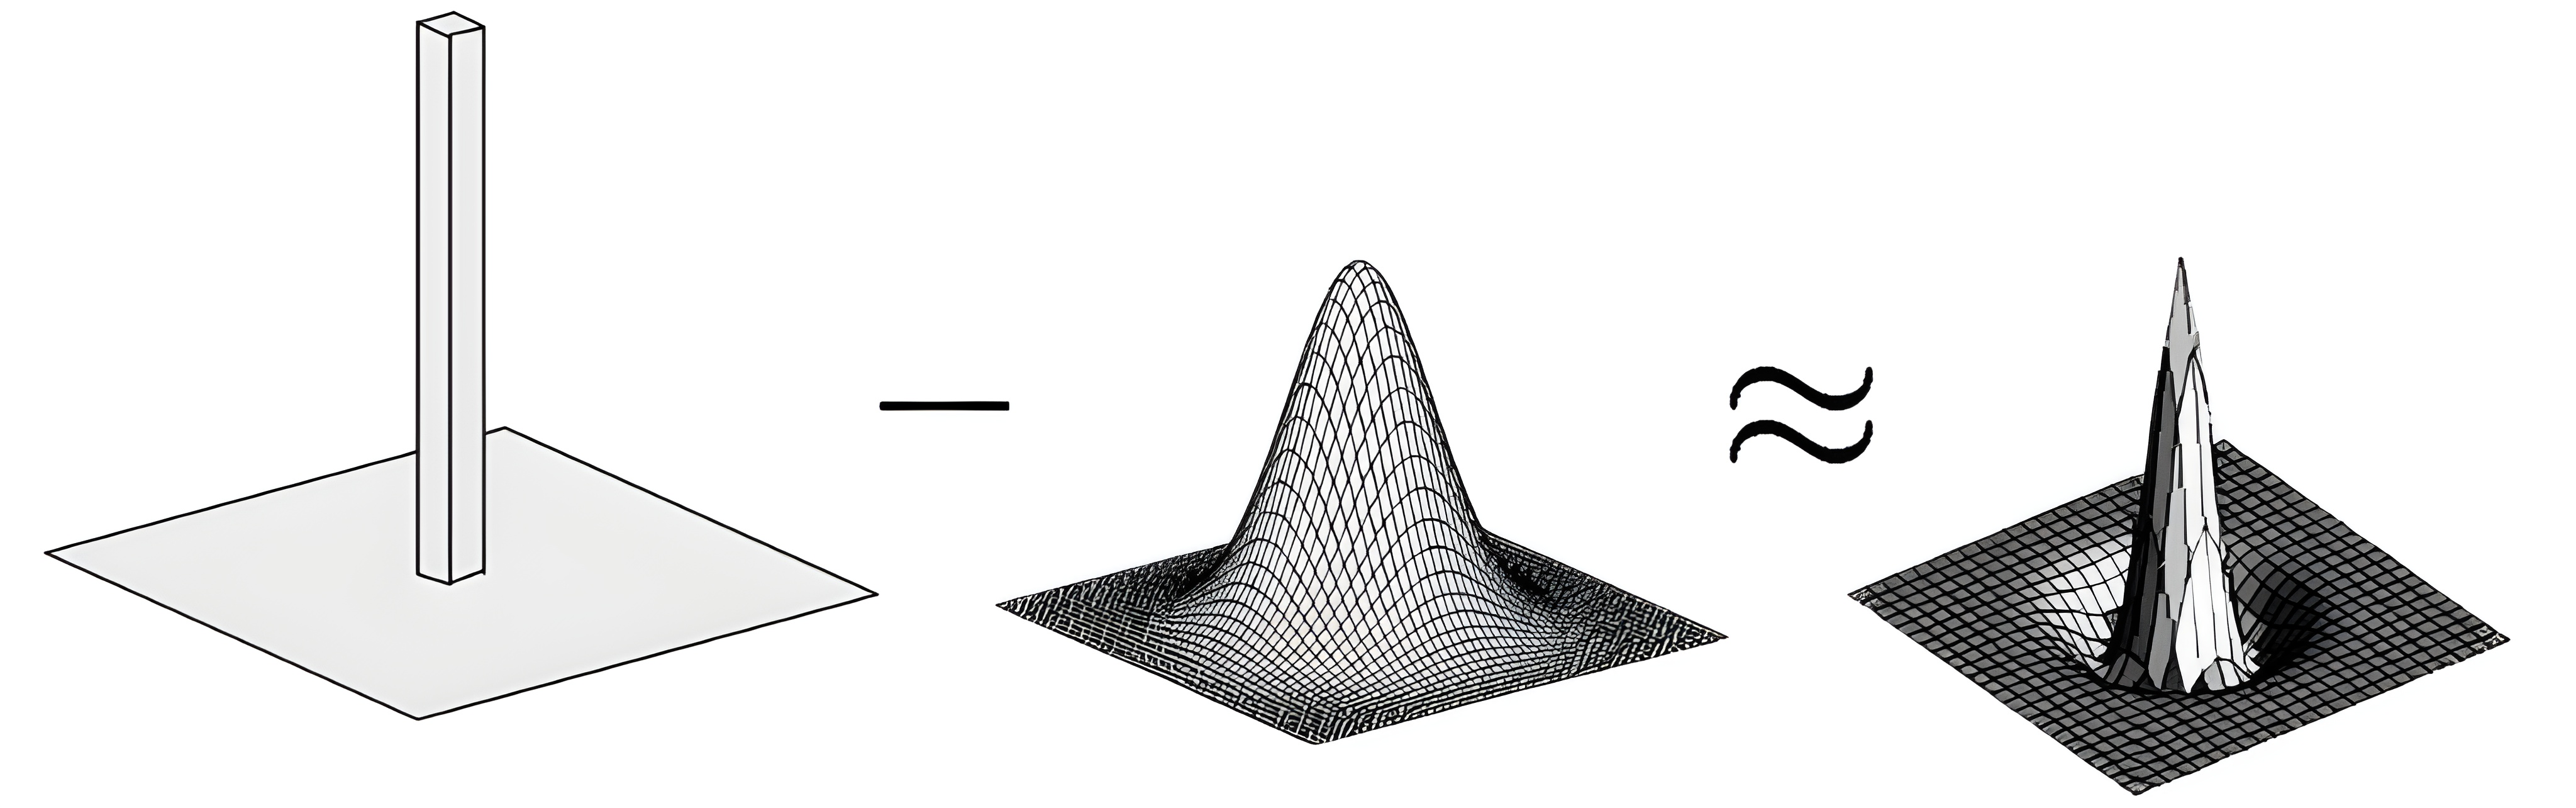
\includegraphics[width=0.63\textwidth ]{images/sharpening_gaussian.png} 
\end{center}
The Gaussian filter works well but have a problem: since it averages also across the edges, these are lost and the image becomes hard to read, too much information are lost. There is a way to give the blurry effects while preserving the edges.
\begin{center}
    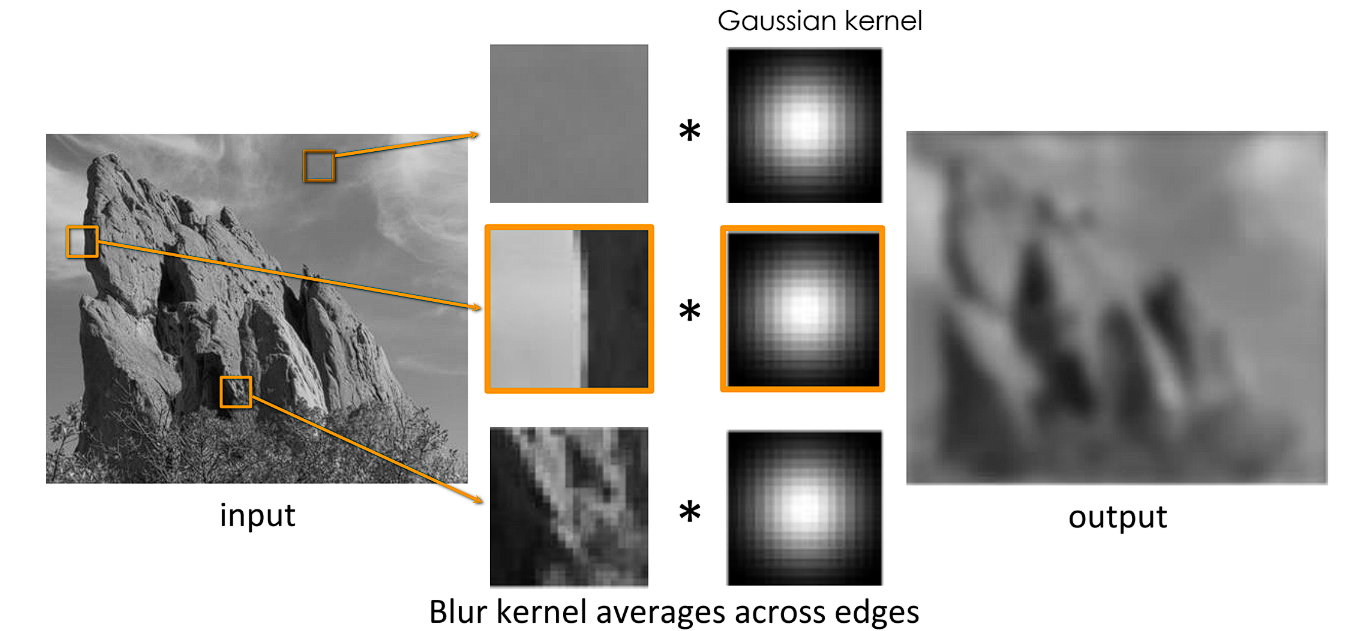
\includegraphics[width=0.7\textwidth ]{images/blur edges.png} 
\end{center}
The \textbf{Bilateral filter} do not blur if there is an edge.
\begin{center}
    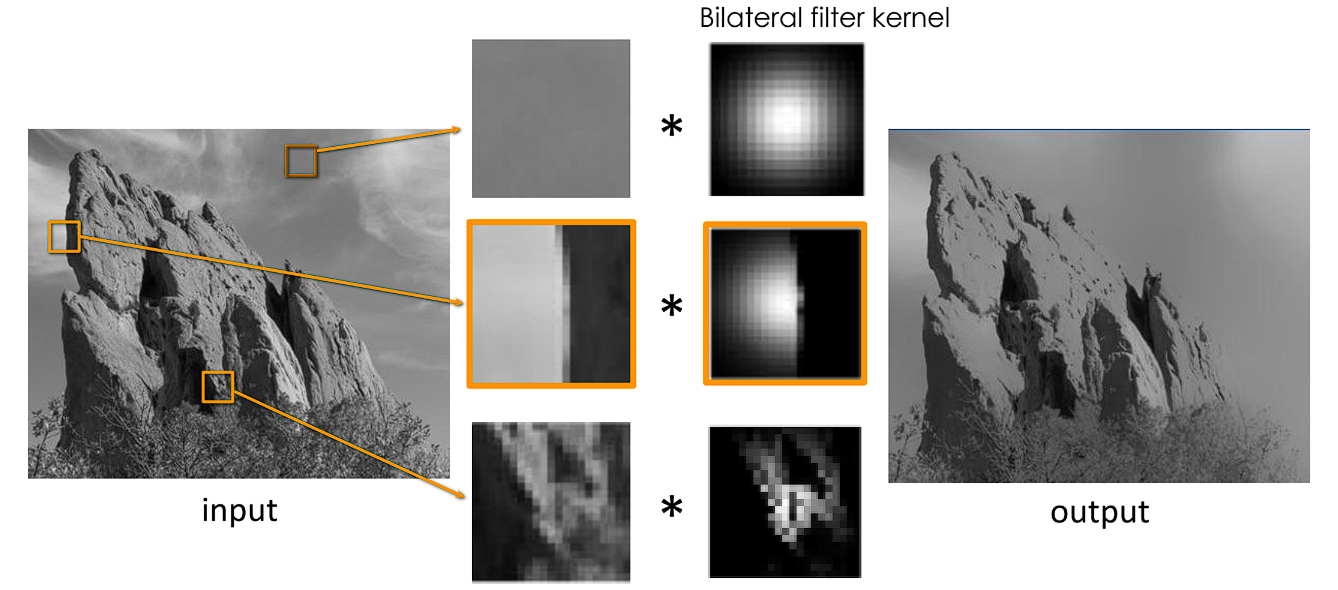
\includegraphics[width=0.7\textwidth ]{images/bilateral.png} 
\end{center}
Is defined as follows: let $f$ to be the original image, and $h$ the result of the filtering\begin{equation}
    h[m,n]=\frac{1}{W_{m,n}}\sum_{k}\sum_lG_\sigma[k,l]r_{m,n}[k,l]f[m+k,n+l]
\end{equation}
where\begin{itemize}
    \item $G_\sigma$ is the Gaussian filter
    \item $W_{m,n}$ is a normalization factor
    \item $r_{m,n}$ is a function defined as follows\begin{equation}
        r_{mn}[k, l] = \exp\left( -\frac{\|f[m, n] - f[m+k, n+l]\|^2}{2\sigma_r^2} \right)
    \end{equation}
    \begin{itemize}
        \item $\sigma_r$ it is the ''intensity range'' parameter indicated in the image. Determines how similar the color of a pixel must be to be considered in the calculation.
        \item If the intensity difference between two pixels is small (the pixels are similar), $r_{mn}$ is close to 1, so the pixel contributes a lot to the average.
        \item If the difference is large (for example, there is a sharp edge), $r_{mn}$ becomes close to 0, effectively excluding that pixel from the calculation.
    \end{itemize}
\end{itemize}
\begin{itemize}
    \item \textbf{Gaussian filtering}: Smooths everything nearby (even edges), only depends on spatial distance
    \item \textbf{Bilateral filtering}: Smooths ''close'' pixels in space and intensity, depends on spatial and intensity distance
\end{itemize}
\begin{center}
    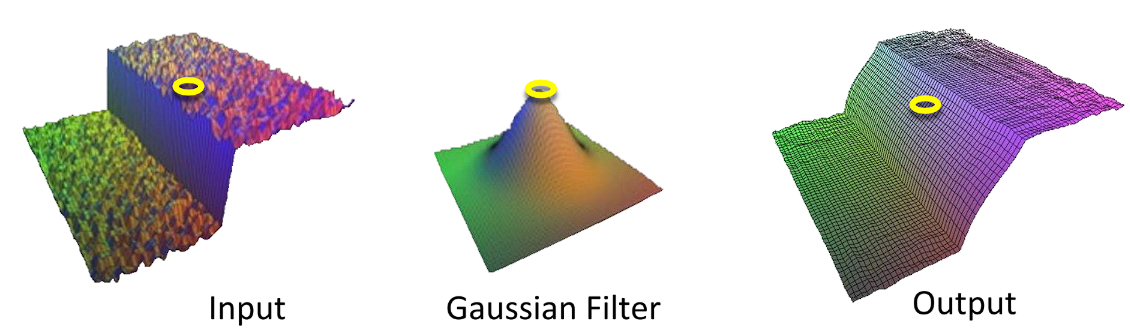
\includegraphics[width=0.7\textwidth ]{images/gaussian_application.png} \\
    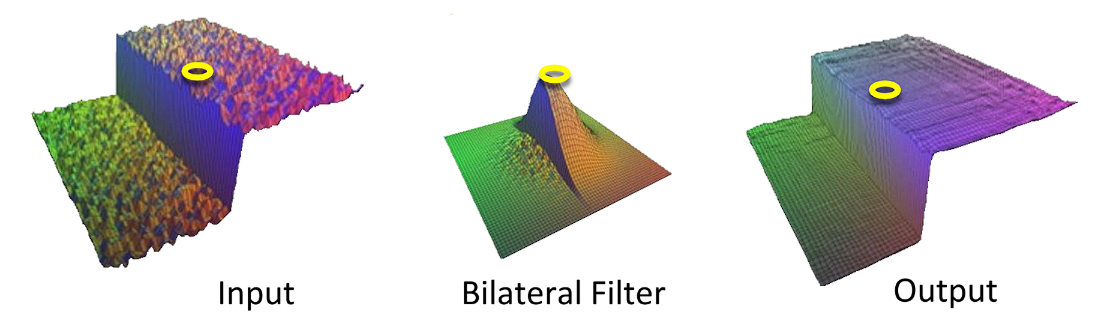
\includegraphics[width=0.7\textwidth ]{images/bilateral_application.png}
\end{center}
If the goal is to enhance contrast while preserving edges, bilateral filtering is generally a better choice. If the goal is to reduce noise or blur the image slightly, Gaussian filtering might be suitable, but it might not
preserve edges as well as bilateral filtering.
\subsection{Sampling and Aliasing}
When we need to reduce the size of an image, we can discard (for example) the odd rows and the odd columns, to reduce in half the resolution, this process is called \textit{sub sampling}.
\begin{center}
    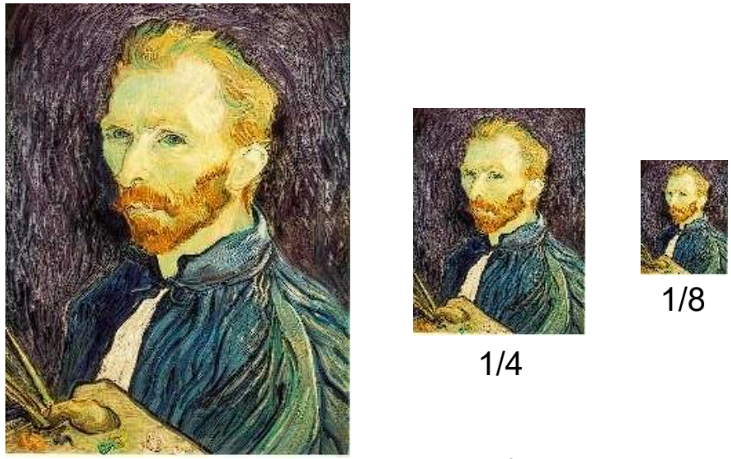
\includegraphics[width=0.4\textwidth ]{images/subsampling.png}
\end{center}
This procedure lost some information, this can be seen since, if we try to zoom the image we will se the \textit{aliasing} effects.
\begin{center}
    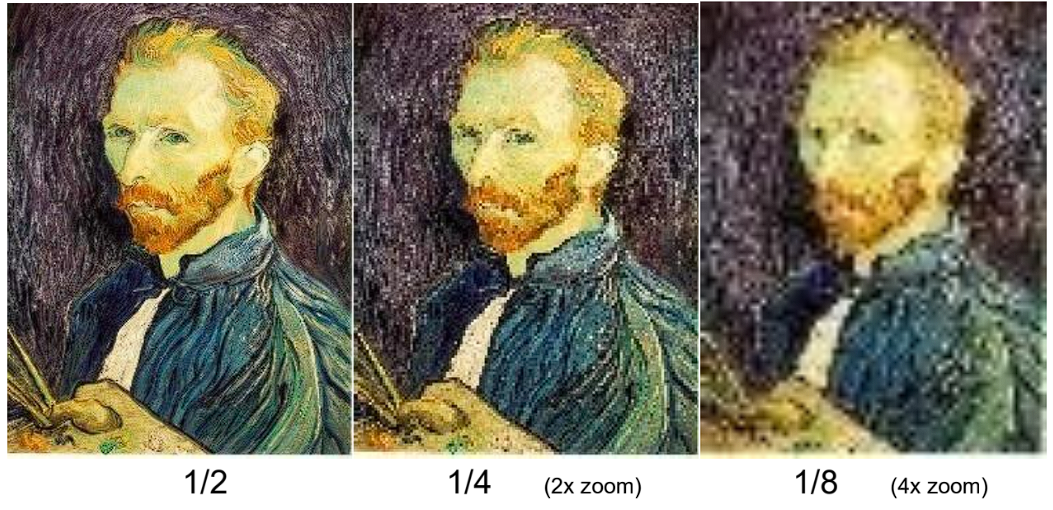
\includegraphics[width=0.6\textwidth ]{images/aliasing.png}
\end{center}
The \textbf{aliasing} occurs when the sampling rate is not high enough to capture the amount of detail in the image, to make a good sampling, we need to understand the structure of an image by frequency analysis, explained in details in Section \ref{frequencyAnalysis}.\bigskip 

To avoid the aliasing, the sampling rate should be greater or at least equal to the double of the max frequency in the image (Nyquist rate).
The Gaussian filter eliminates the higher frequencies in an image, so a basic idea of sampling is to apply this low pass filter: We filter the image with a Gaussian filter, and then sub sample.
\begin{center}
    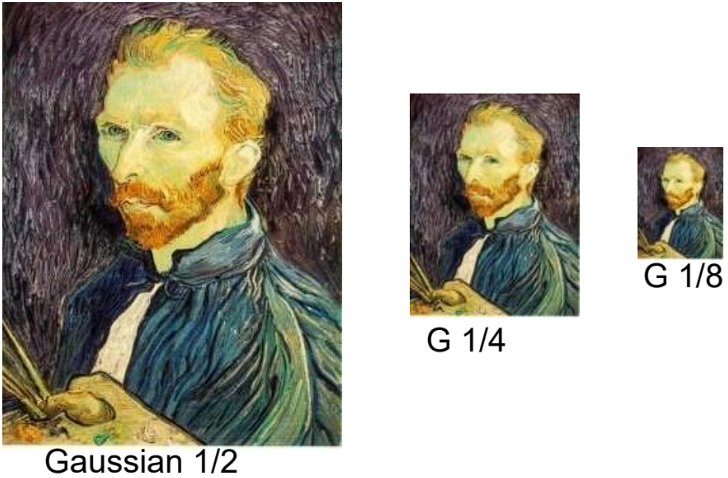
\includegraphics[width=0.4\textwidth ]{images/subsampling_gaussian.png}
\end{center}
\begin{center}
    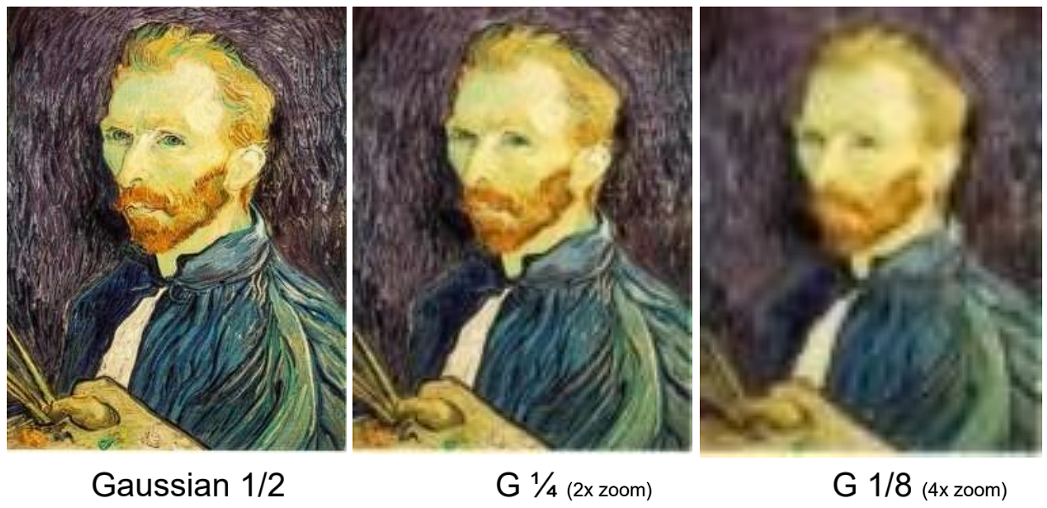
\includegraphics[width=0.6\textwidth ]{images/aliasing_gaussian.png}
\end{center}
If we iteratively apply this filter-sampling procedure, we get a sequence of images, where each image has half the resolution of the previous one, this series is called \textbf{Gaussian Pyramid}.
\begin{center}
    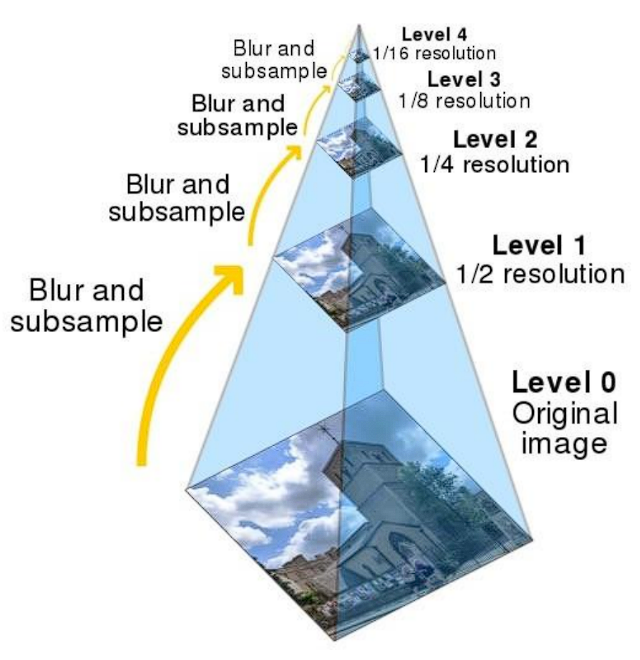
\includegraphics[width=0.3\textwidth ]{images/gaussian_pyramid.png}
\end{center}
The \textbf{upsampling} procedure is the opposite of the down sampling: We take an image and we repeat $n$ times each column (to increase the resolution of a factor $n$), this method is called nearest neighbor
interpolation.
\begin{center}
    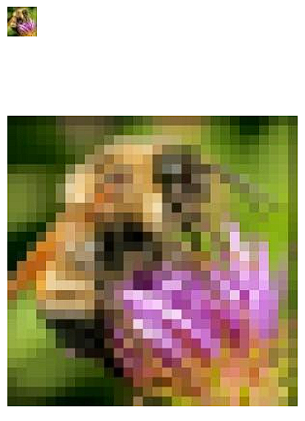
\includegraphics[width=0.2\textwidth ]{images/upsampling.png}
\end{center}
There are also other methods, like the bilinear interpolation and the bicubic interpolation.
\begin{center}
    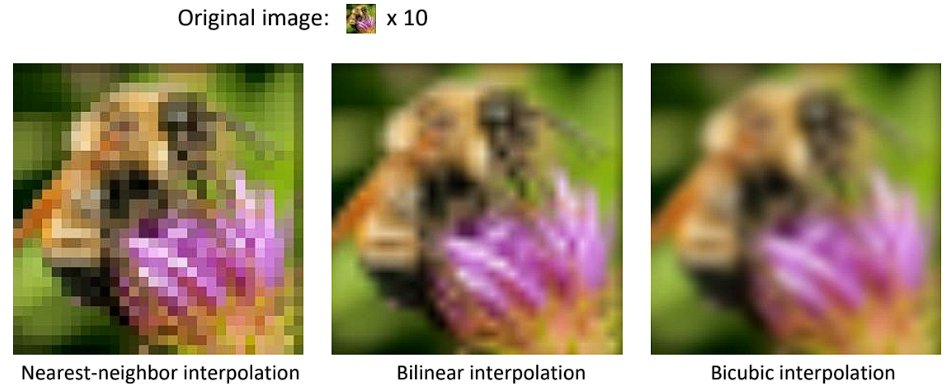
\includegraphics[width=0.6\textwidth ]{images/upsampling2.png}
\end{center}
The bilinear interpolation is computationally less intensive and faster than bicubic interpolation. If speed is a critical factor, bilinear interpolation might be preferred. Bicubic interpolation generally provides smoother and more accurate results, making it suitable for applications where image quality is a priority.\begin{itemize}
    \item Bilinear interpolation calculates the value of the new pixel by taking a weighted average of the 4 neighboring pixels (2x2).
    \item Bicubic interpolation is more complex and precise: it calculates the value of the new pixel by analyzing the 16 surrounding pixels (4x4). Uses cubic polynomials to create a smooth curve between pixel values. Instead of drawing straight lines between the dots, try to follow the flow of colors and contrasts.
\end{itemize}
\begin{center}
    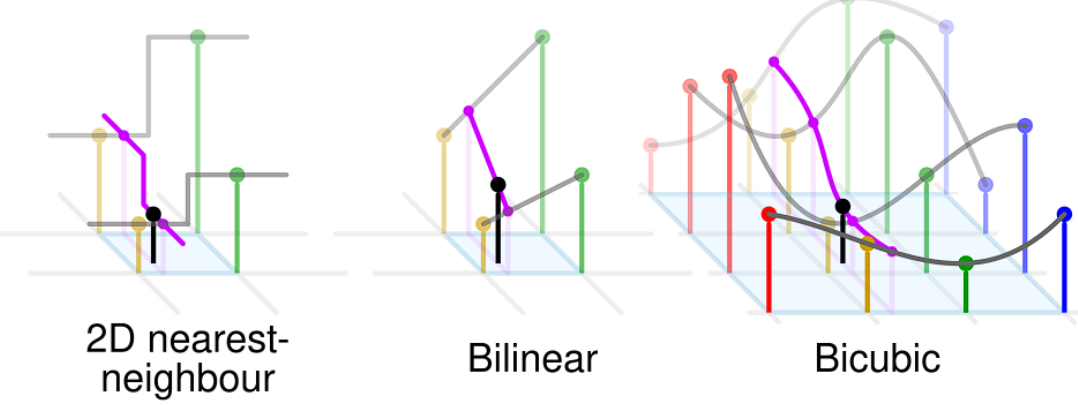
\includegraphics[width=0.6\textwidth ]{images/bilinear_bicubic.png}
\end{center}
\section{Image Derivatives}
An image is a discrete sampling of a function $f:\R^2\rightarrow\R$ (in practice, there are three functions, one for each channel). The partial derivative formula for a continuous function:\begin{equation}
    \frac{\partial f(x,y)}{\partial x}=\lim_{\epsilon\rightarrow 0}\frac{f(x+\epsilon,y)-f(x,y)}{\epsilon}
\end{equation}
can be approximated by a finite difference for our discrete images:\begin{align}
    &\frac{\partial f(x,y)}{\partial x}\simeq \frac{f(x+1,y)-f(x,y)}{1}\\
    &\frac{\partial f(x,y)}{\partial x}\simeq \frac{f(x+1,y)-f(x-1,y)}{2}
\end{align}
these operation can be realized by two kernels:\begin{center}
    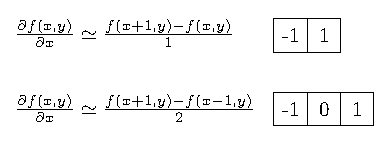
\includegraphics[width=0.4\textwidth ]{images/derivatives.eps}
\end{center}
Similarly, the derivative respect to $y$ can be approximated by the same kernel but transposed:
\begin{center}
    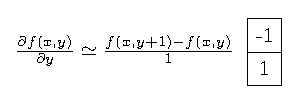
\includegraphics[width=0.4\textwidth ]{images/derivatives2.eps}
\end{center}
By applying the convolution we can compute the two derivatives of an image, called the \textbf{gradient}:
\begin{center}
    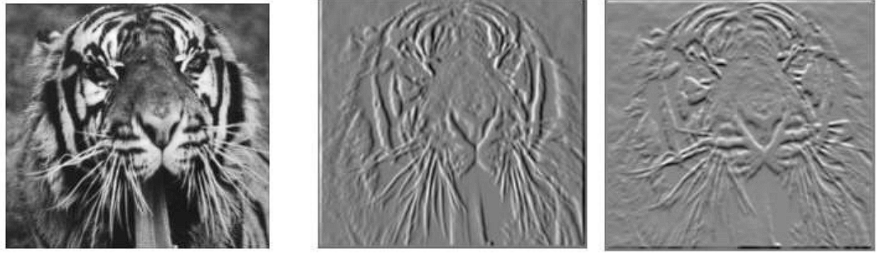
\includegraphics[width=0.6\textwidth ]{images/derivatives3.png}
\end{center}
we can also display the norm of the gradient\begin{equation}
    \|\nabla f\|=\sqrt{\left(\frac{\partial f}{\partial x}\right)^2+\left(\frac{\partial f}{\partial y}\right)^2}.
\end{equation}
\begin{center}
    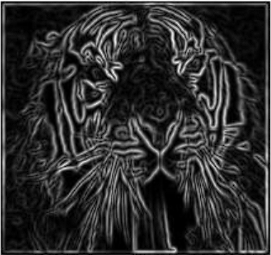
\includegraphics[width=0.2\textwidth ]{images/gradient}
\end{center}
The gradient is a vector that points in the direction of most rapid increase in the intensity, and the strength of this increase is given by the norm. The gradient direction is given by\begin{equation}\label{dir_grad}
    \theta=\tan^{-1}\left(\frac{\nicefrac{\partial f}{\partial y}}{\nicefrac{\partial f}{\partial x}}\right),
\end{equation}
\subsection{Edge Detection}
The goal of the edge detection is to convert a 2D image in a set of curves, extracting salient features in the scene, to represent it in a more compact way respect to the pixels. If we represent the intensity of a grey scale image in the $z$ axis of a plot, the edges will look like steep cliff.
\begin{center}
    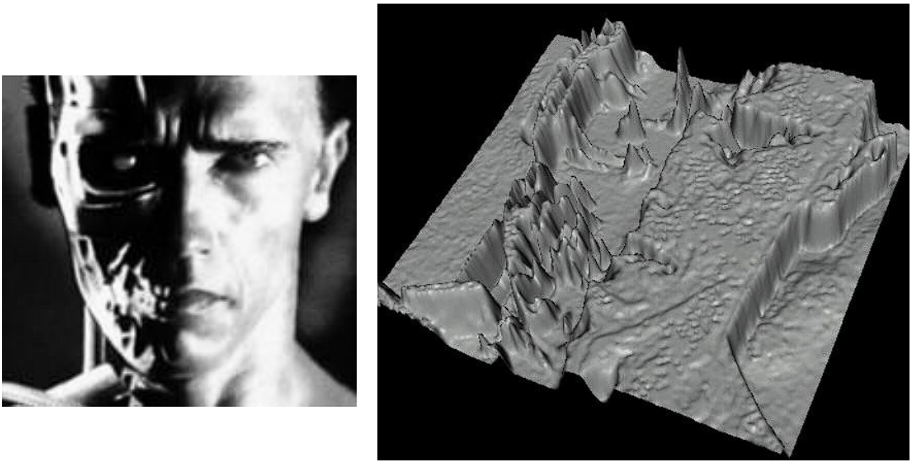
\includegraphics[width=0.6\textwidth ]{images/edges.png}
\end{center}
In general, an edge is a \textit{rapid change} in the image intensity function. We can consider a \textit{scan line} in the 2D image, and plot the intensity along this line, to get a one dimensional signal:
\begin{center}
    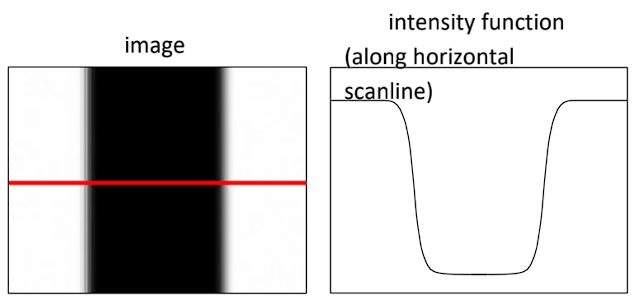
\includegraphics[width=0.6\textwidth ]{images/scanline.png}
\end{center}
here the edges can be seen clearly, if we consider the derivative of this signal, the edges will corresponds to local maxima and/or minima. The direction of the edges is given by the direction of the gradient, computed like in the equation \eqref{dir_grad}.\bigskip

If an image is noisy, it may be difficult to detect the edge through the derivative, like in the following example:
\begin{center}
    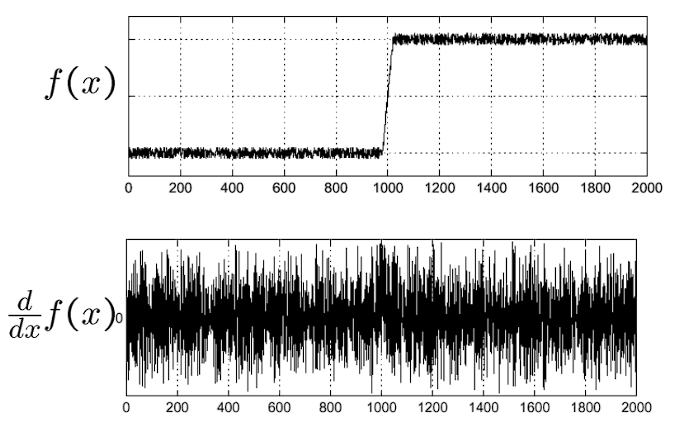
\includegraphics[width=0.5\textwidth ]{images/noisy_der.png}
\end{center}
To solve this problem we need to apply a smoothening filter to the image, the convolution with a Gaussian kernel will solve the problem and make easier to find the edges.
\begin{center}
    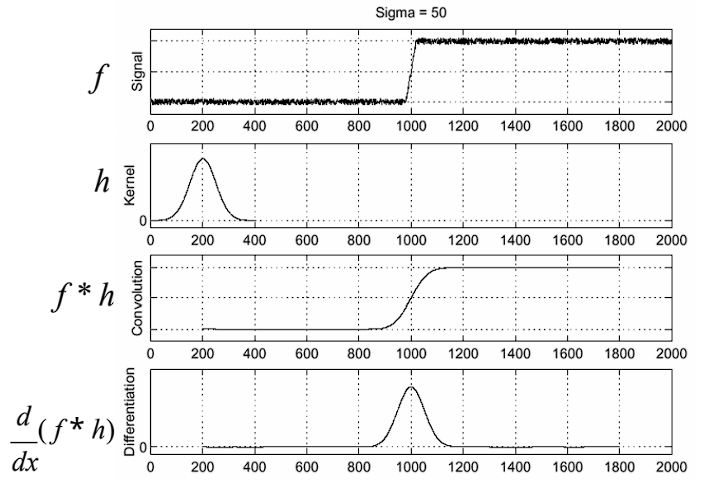
\includegraphics[width=0.5\textwidth ]{images/edge_gaussian.png}
\end{center}
\begin{boxtheorem}{Derivative Theorem of Convolution}{}
The derivative of the convolution between $f$ and $h$ is equal to the derivative of $h$ convolved with $f$:\begin{equation}
    \frac{(\partial h\star f)}{\partial x}=\left(\frac{\partial h}{\partial x}\right)\star f
    .
\end{equation}
\end{boxtheorem}
Instead of computing the derivative of the convolution, we can exploit the derivative theorem of convolution to save time and do less steps to compute $\frac{d}{dx}(f\star h)$.
\begin{center}
    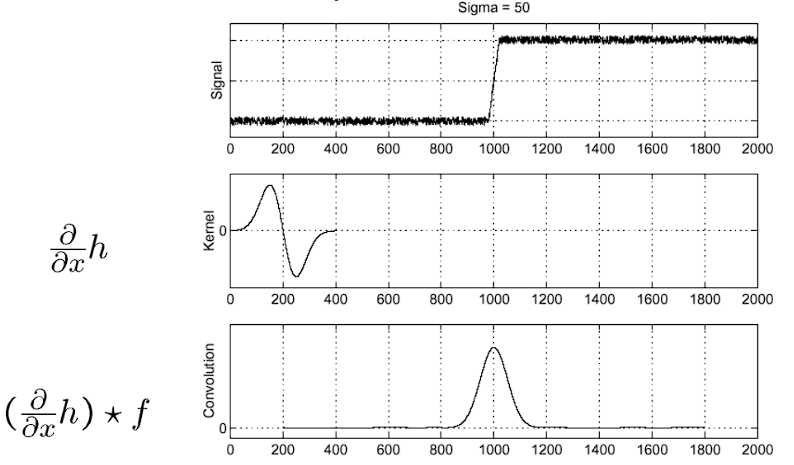
\includegraphics[width=0.5\textwidth ]{images/edge_gaussian2.png}
\end{center}
So instead of considering the Gaussian filter we consider the derivative of it in both directions.
\begin{center}
    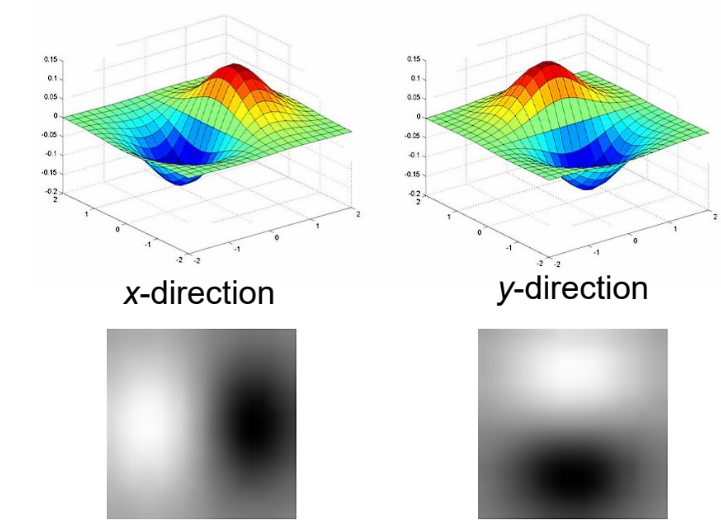
\includegraphics[width=0.4\textwidth ]{images/derivative_of_gaussian.png}
\end{center}
As we have seen, the first derivative 1D filter\begin{equation}
    \begin{bmatrix}
        1&0&-1
    \end{bmatrix}
\end{equation}
comes from a first order finite difference approximation of a partial derivative. We can consider a second order finite difference to approximate the second derivative, this leads to the \textbf{Laplace filter}:\begin{equation}\label{laplace_filter}
    \begin{bmatrix}
        1&-2&1
    \end{bmatrix}
\end{equation}
So, we can derive two times the Gaussian filter, this approximation is called \textbf{Laplacian of Gaussian (LoG) filter}, is given by the convolution of the Gaussian filter in equation \eqref{gaussian_filter} with the 1D Laplace filter given in equation \eqref{laplace_filter}.\bigskip 

If we apply this LoG filter to a function we will get a signal that, \textit{crosses the zero} on the edges.
\begin{center}
    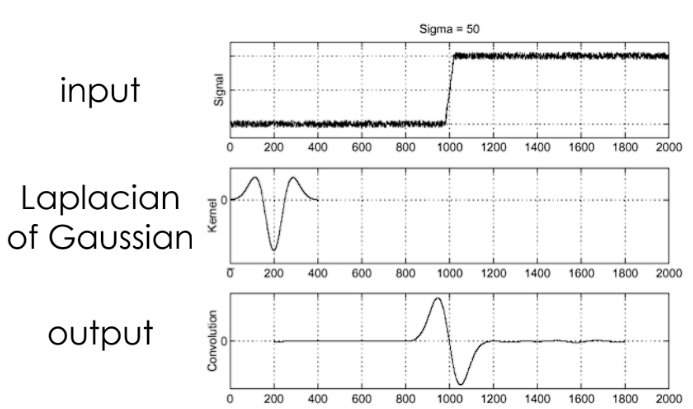
\includegraphics[width=0.5\textwidth ]{images/LoG.png}
\end{center}
\begin{center}
    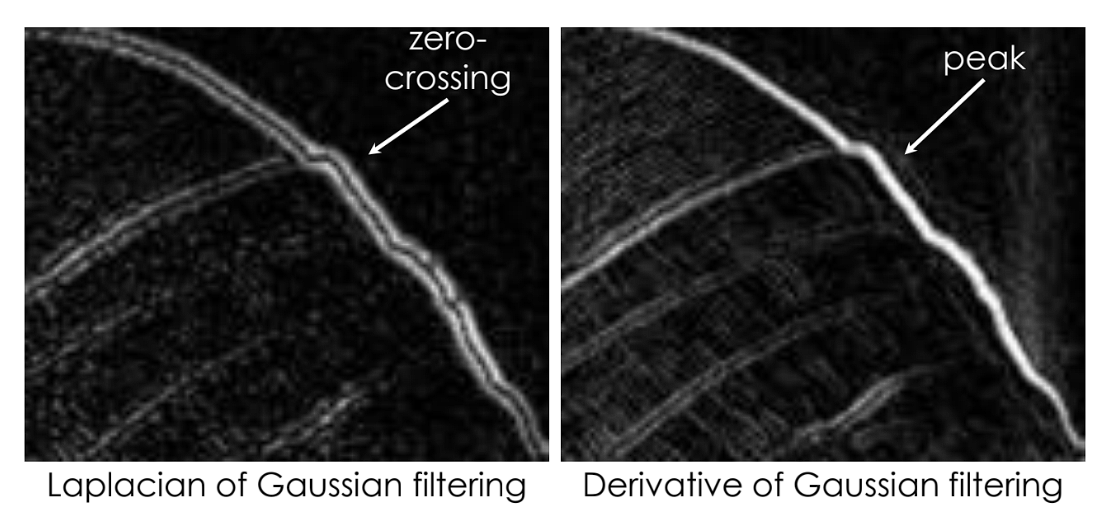
\includegraphics[width=0.5\textwidth ]{images/LoG2.png}
\end{center}
The zero crossing LoG procedure is more accurate at localizing the edges, but the derivative of Gaussian method is more efficient and fast to compute.\bigskip

An approximation of the derivative of Gaussian filter is given by the \textbf{Sobel filter}:\begin{equation}
    s_x=\frac{1}{8}\begin{bmatrix}
        -1&0&1\\
        -2&0&2\\
        -1&0&1
    \end{bmatrix} \ \ \ \ \ \  
     s_y=\frac{1}{8}\begin{bmatrix}
        1&2&1\\
        0&0&0\\
        -1&-2&-1
    \end{bmatrix}
\end{equation}
$s_x$ is the horizontal sobel filter while $s_y$ is the vertical sobel filter. These filters are separable:\begin{align}
    &s_x=\begin{bmatrix}
        1\\2\\1
    \end{bmatrix}\cdot \begin{bmatrix}
        1&0&-1
    \end{bmatrix}\\ 
    &s_y=\begin{bmatrix}
        1\\0\\-1
    \end{bmatrix}\cdot \begin{bmatrix}
        1&2&1
    \end{bmatrix}
\end{align}
\begin{center}
    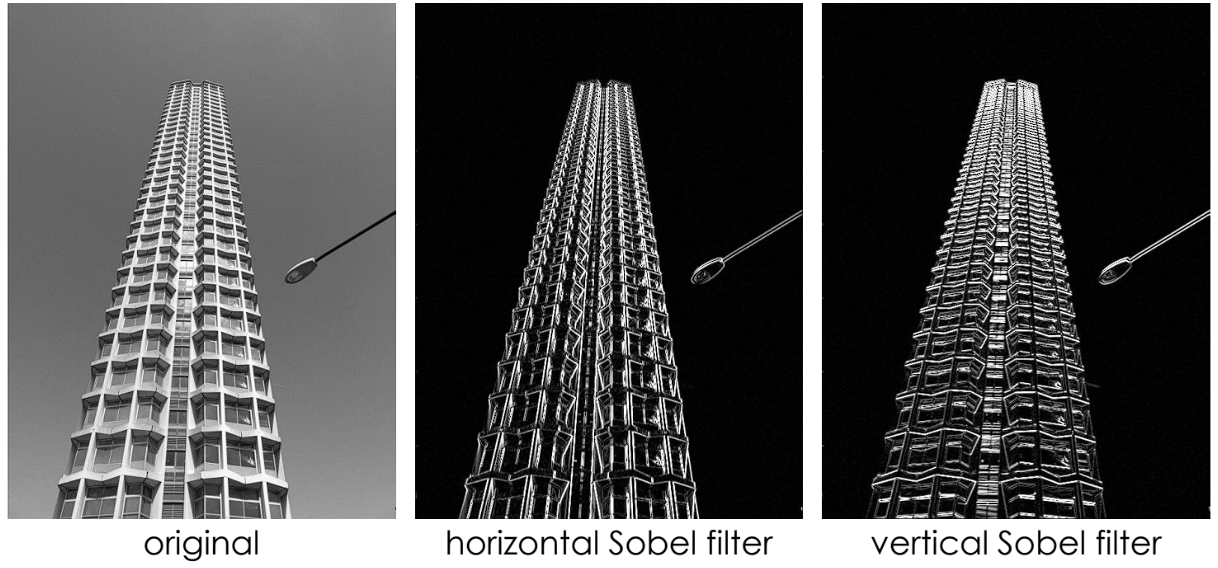
\includegraphics[width=0.6\textwidth ]{images/sobel.png}
\end{center}
\subsection{Canny Edge Detector}
An optimal edge detector should\begin{itemize}
    \item be accurate, minimize the number of false positives and false negatives 
    \item have precise localization, pinpointing edges at the
positions where they actually occur
\item have single response, ensuring that only
one edge is found where there only is one edge.
\end{itemize}
A good procedure is the \textbf{Non-Maximum Suppression}: Let's consider the following image
\begin{center}
    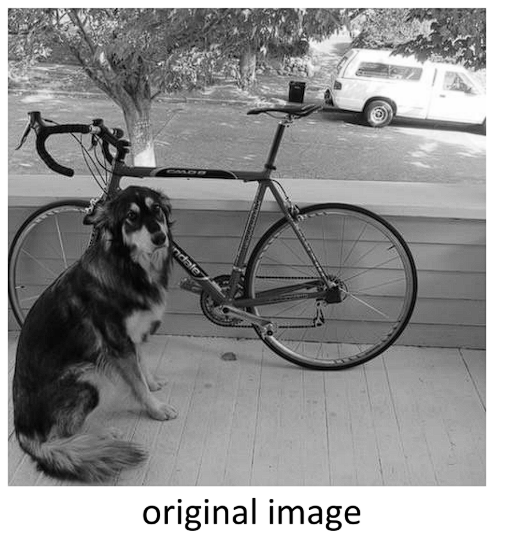
\includegraphics[width=0.3\textwidth ]{images/dog_image.png}
\end{center}
to localize the edges we try to smooth the image and then consider the norm of the gradient
\begin{center}
    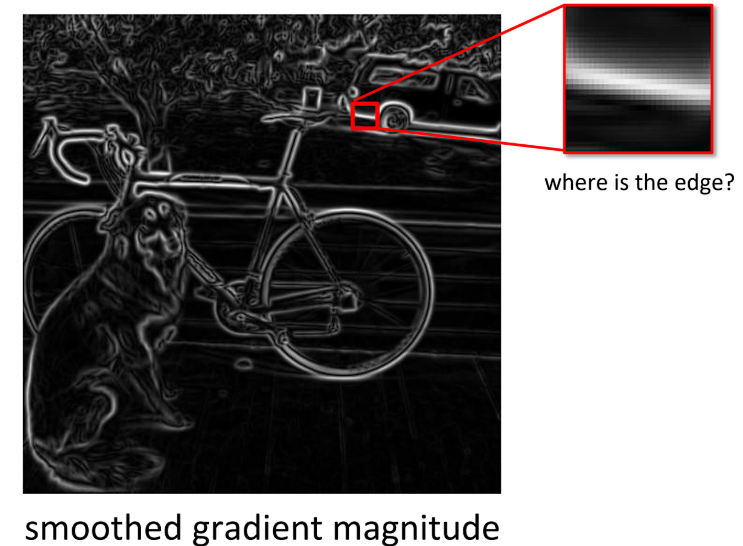
\includegraphics[width=0.43\textwidth ]{images/dog_image2.png}
\end{center}
It is hard to localize precisely the edge, since we get a wide line of pixels of different intensity. To find the perfect 1-pixel wide edge, we may look at the intensity along the direction of the gradient.
We can get the orientation angle for each pixel:
\begin{center}
    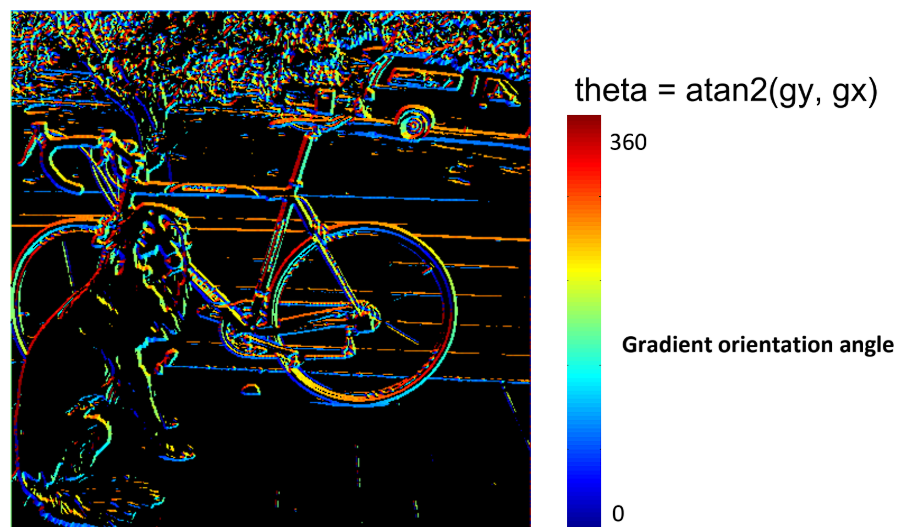
\includegraphics[width=0.43\textwidth ]{images/dog_image3.png}
\end{center}
The procedure is the following\begin{enumerate}
    \item for each pixel, we compute the direction of the gradient in that point
    \item we compare the intensity of that pixel with the local neighbors along the direction of the gradient
    \item if the current pixel is the most intense among its neighbors in the direction of the gradient, it is retained. Otherwise, it is suppressed: The intensity is set to zero.
\end{enumerate}

\begin{center}
    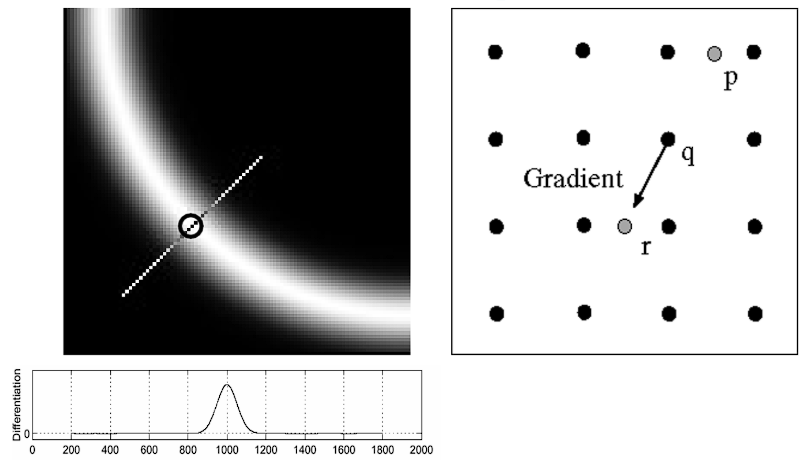
\includegraphics[width=0.5\textwidth ]{images/nonmaxsupp.png}
\end{center}
The following image is the result of the Non-Max Suppression:
\begin{center}
    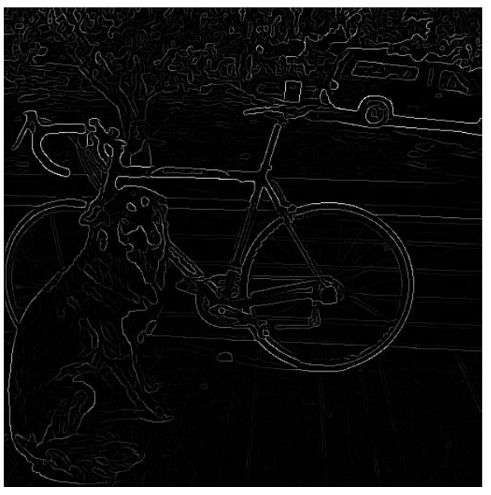
\includegraphics[width=0.3\textwidth ]{images/dog_image4.png}
\end{center}
Of course, there is some noise left, we want to keep only the strong edges, we can consider two thresholds $t$ and $T$, for each pixel:\begin{itemize}
    \item let $R$ to be the intensity of the gradient of the inspected pixel 
    \item if $R>T$, the pixel is on a strong edge 
    \item if $t<R<T$, the pixel is on a weak edge 
    \item if $R<t$, it's not an edge 
\end{itemize}
we can keep the strong edges and the weak edges that connects to strong edges, by looking at the 8 closest neighbors. It is important to tune correctly $t$ and $T$. This stage also removes small pixels noises on the assumption that edges are long lines.\bigskip 

The \textbf{Edge Tracking by Hysteresis} consists in transforming weak pixels into strong one if and only if at least one pixels around the one being processed is a strong
one.
\begin{center}
    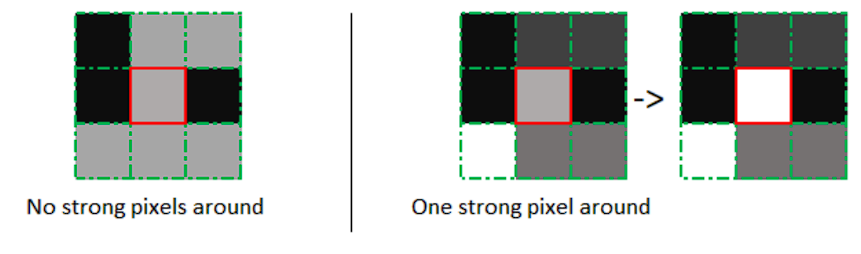
\includegraphics[width=0.4\textwidth ]{images/Hysteresis.png}
\end{center}
Summing up all the steps described, we arrive at the \textbf{Canny Edge Detector}, characterized by the following steps:\begin{enumerate}
    \item Filter image with Derivative of Gaussian.
    \item Find magnitude and orientation of gradient.
    \item Non-maximum suppression.
    \item Linking and thresholding (hysteresis)\begin{itemize}
        \item define a low threshold $t$ and an high threshold $T$
        \item use the high threshold to start edge curves and the
low threshold to continue them.
    \end{itemize}
\end{enumerate}
The results of the Canny edge detector depends on the choice of the thresholds and the Gaussian blur $\sigma$.
\begin{center}
    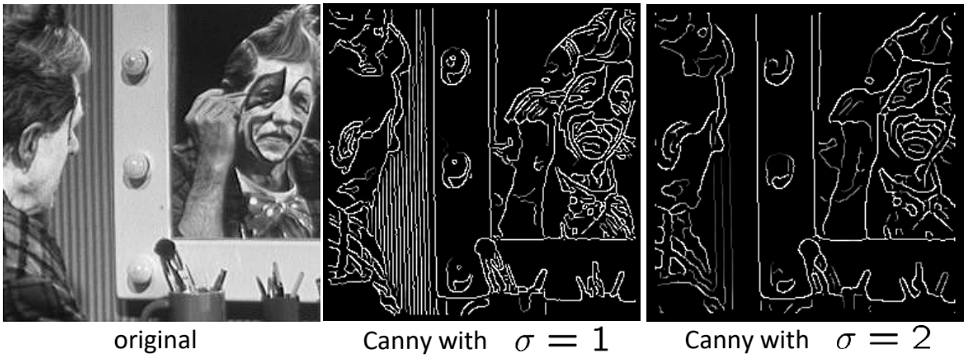
\includegraphics[width=0.6\textwidth ]{images/canny.png}
\end{center}
\section{Image Pyramids}







\newpage
\section{Frequency Analysis}\label{frequencyAnalysis}
\redText{TODO}
\end{document}